\documentclass[1p]{elsarticle_modified}
%\bibliographystyle{elsarticle-num}

%\usepackage[colorlinks]{hyperref}
%\usepackage{abbrmath_seonhwa} %\Abb, \Ascr, \Acal ,\Abf, \Afrak
\usepackage{amsfonts}
\usepackage{amssymb}
\usepackage{amsmath}
\usepackage{amsthm}
\usepackage{scalefnt}
\usepackage{amsbsy}
\usepackage{kotex}
\usepackage{caption}
\usepackage{subfig}
\usepackage{color}
\usepackage{graphicx}
\usepackage{xcolor} %% white, black, red, green, blue, cyan, magenta, yellow
\usepackage{float}
\usepackage{setspace}
\usepackage{hyperref}

\usepackage{tikz}
\usetikzlibrary{arrows}

\usepackage{multirow}
\usepackage{array} % fixed length table
\usepackage{hhline}

%%%%%%%%%%%%%%%%%%%%%
\makeatletter
\renewcommand*\env@matrix[1][\arraystretch]{%
	\edef\arraystretch{#1}%
	\hskip -\arraycolsep
	\let\@ifnextchar\new@ifnextchar
	\array{*\c@MaxMatrixCols c}}
\makeatother %https://tex.stackexchange.com/questions/14071/how-can-i-increase-the-line-spacing-in-a-matrix
%%%%%%%%%%%%%%%

\usepackage[normalem]{ulem}

\newcommand{\msout}[1]{\ifmmode\text{\sout{\ensuremath{#1}}}\else\sout{#1}\fi}
%SOURCE: \msout is \stkout macro in https://tex.stackexchange.com/questions/20609/strikeout-in-math-mode

\newcommand{\cancel}[1]{
	\ifmmode
	{\color{red}\msout{#1}}
	\else
	{\color{red}\sout{#1}}
	\fi
}

\newcommand{\add}[1]{
	{\color{blue}\uwave{#1}}
}

\newcommand{\replace}[2]{
	\ifmmode
	{\color{red}\msout{#1}}{\color{blue}\uwave{#2}}
	\else
	{\color{red}\sout{#1}}{\color{blue}\uwave{#2}}
	\fi
}

\newcommand{\Sol}{\mathcal{S}} %segment
\newcommand{\D}{D} %diagram
\newcommand{\A}{\mathcal{A}} %arc


%%%%%%%%%%%%%%%%%%%%%%%%%%%%%5 test

\def\sl{\operatorname{\textup{SL}}(2,\Cbb)}
\def\psl{\operatorname{\textup{PSL}}(2,\Cbb)}
\def\quan{\mkern 1mu \triangleright \mkern 1mu}

\theoremstyle{definition}
\newtheorem{thm}{Theorem}[section]
\newtheorem{prop}[thm]{Proposition}
\newtheorem{lem}[thm]{Lemma}
\newtheorem{ques}[thm]{Question}
\newtheorem{cor}[thm]{Corollary}
\newtheorem{defn}[thm]{Definition}
\newtheorem{exam}[thm]{Example}
\newtheorem{rmk}[thm]{Remark}
\newtheorem{alg}[thm]{Algorithm}

\newcommand{\I}{\sqrt{-1}}
\begin{document}

%\begin{frontmatter}
%
%\title{Boundary parabolic representations of knots up to 8 crossings}
%
%%% Group authors per affiliation:
%\author{Yunhi Cho} 
%\address{Department of Mathematics, University of Seoul, Seoul, Korea}
%\ead{yhcho@uos.ac.kr}
%
%
%\author{Seonhwa Kim} %\fnref{s_kim}}
%\address{Center for Geometry and Physics, Institute for Basic Science, Pohang, 37673, Korea}
%\ead{ryeona17@ibs.re.kr}
%
%\author{Hyuk Kim}
%\address{Department of Mathematical Sciences, Seoul National University, Seoul 08826, Korea}
%\ead{hyukkim@snu.ac.kr}
%
%\author{Seokbeom Yoon}
%\address{Department of Mathematical Sciences, Seoul National University, Seoul, 08826,  Korea}
%\ead{sbyoon15@snu.ac.kr}
%
%\begin{abstract}
%We find all boundary parabolic representation of knots up to 8 crossings.
%
%\end{abstract}
%\begin{keyword}
%    \MSC[2010] 57M25 
%\end{keyword}
%
%\end{frontmatter}

%\linenumbers
%\tableofcontents
%
\newcommand\colored[1]{\textcolor{white}{\rule[-0.35ex]{0.8em}{1.4ex}}\kern-0.8em\color{red} #1}%
%\newcommand\colored[1]{\textcolor{white}{ #1}\kern-2.17ex	\textcolor{white}{ #1}\kern-1.81ex	\textcolor{white}{ #1}\kern-2.15ex\color{red}#1	}

{\Large $\underline{12n_{0551}~(K12n_{0551})}$}

\setlength{\tabcolsep}{10pt}
\renewcommand{\arraystretch}{1.6}
\vspace{1cm}\begin{tabular}{m{100pt}>{\centering\arraybackslash}m{274pt}}
\multirow{5}{120pt}{
	\centering
	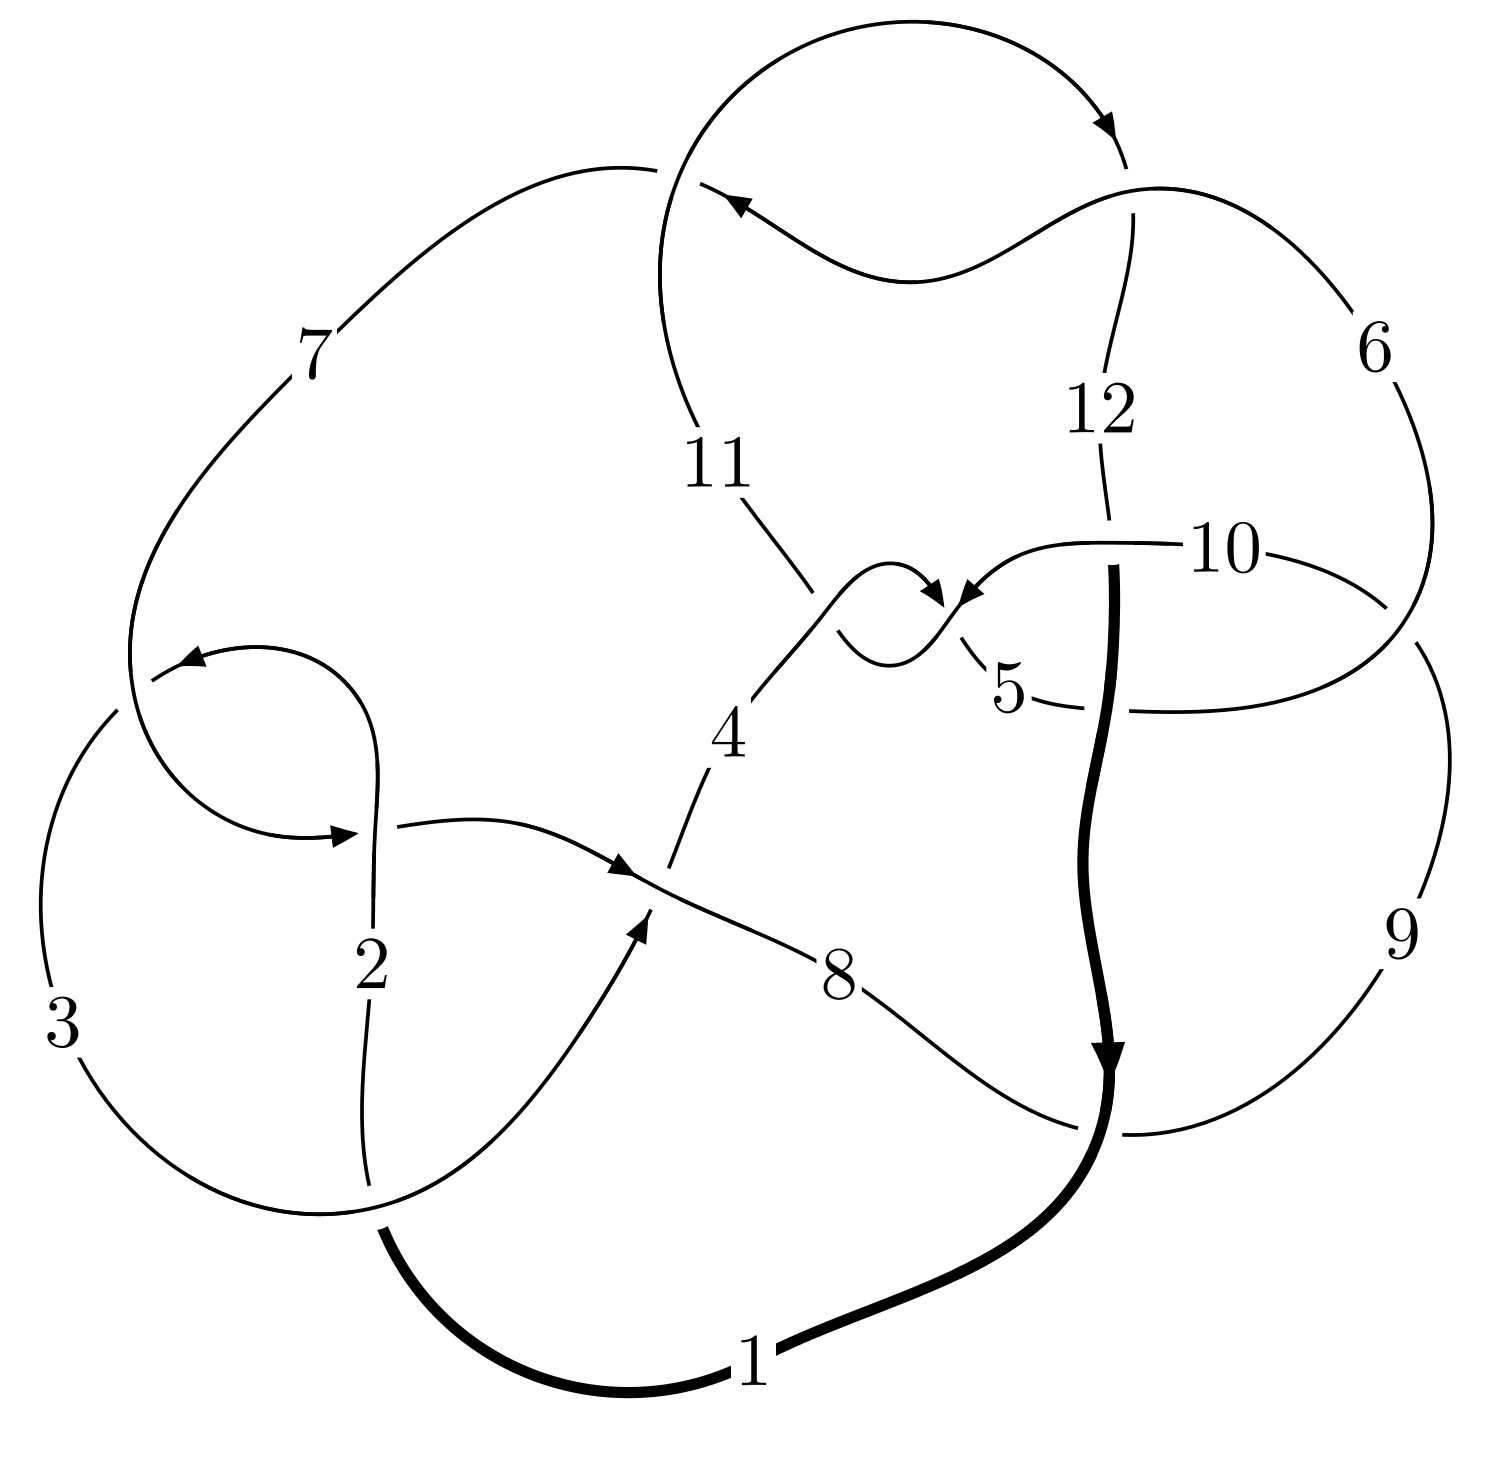
\includegraphics[width=112pt]{../../../GIT/diagram.site/Diagrams/png/2640_12n_0551.png}\\
\ \ \ A knot diagram\footnotemark}&
\allowdisplaybreaks
\textbf{Linearized knot diagam} \\
\cline{2-2}
 &
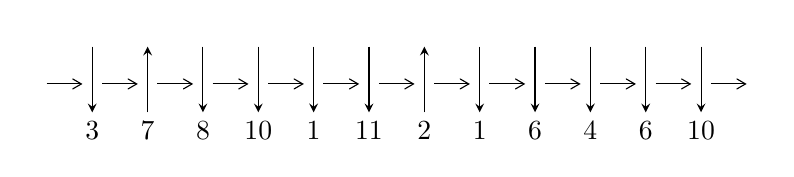
\begin{tikzpicture}[x=20pt, y=17pt]
	% nodes
	\node (C0) at (0, 0) {};
	\node (C1) at (1, 0) {};
	\node (C1U) at (1, +1) {};
	\node (C1D) at (1, -1) {3};

	\node (C2) at (2, 0) {};
	\node (C2U) at (2, +1) {};
	\node (C2D) at (2, -1) {7};

	\node (C3) at (3, 0) {};
	\node (C3U) at (3, +1) {};
	\node (C3D) at (3, -1) {8};

	\node (C4) at (4, 0) {};
	\node (C4U) at (4, +1) {};
	\node (C4D) at (4, -1) {10};

	\node (C5) at (5, 0) {};
	\node (C5U) at (5, +1) {};
	\node (C5D) at (5, -1) {1};

	\node (C6) at (6, 0) {};
	\node (C6U) at (6, +1) {};
	\node (C6D) at (6, -1) {11};

	\node (C7) at (7, 0) {};
	\node (C7U) at (7, +1) {};
	\node (C7D) at (7, -1) {2};

	\node (C8) at (8, 0) {};
	\node (C8U) at (8, +1) {};
	\node (C8D) at (8, -1) {1};

	\node (C9) at (9, 0) {};
	\node (C9U) at (9, +1) {};
	\node (C9D) at (9, -1) {6};

	\node (C10) at (10, 0) {};
	\node (C10U) at (10, +1) {};
	\node (C10D) at (10, -1) {4};

	\node (C11) at (11, 0) {};
	\node (C11U) at (11, +1) {};
	\node (C11D) at (11, -1) {6};

	\node (C12) at (12, 0) {};
	\node (C12U) at (12, +1) {};
	\node (C12D) at (12, -1) {10};
	\node (C13) at (13, 0) {};

	% arrows
	\draw[->,>={angle 60}]
	(C0) edge (C1) (C1) edge (C2) (C2) edge (C3) (C3) edge (C4) (C4) edge (C5) (C5) edge (C6) (C6) edge (C7) (C7) edge (C8) (C8) edge (C9) (C9) edge (C10) (C10) edge (C11) (C11) edge (C12) (C12) edge (C13) ;	\draw[->,>=stealth]
	(C1U) edge (C1D) (C2D) edge (C2U) (C3U) edge (C3D) (C4U) edge (C4D) (C5U) edge (C5D) (C6U) edge (C6D) (C7D) edge (C7U) (C8U) edge (C8D) (C9U) edge (C9D) (C10U) edge (C10D) (C11U) edge (C11D) (C12U) edge (C12D) ;
	\end{tikzpicture} \\
\hhline{~~} \\& 
\textbf{Solving Sequence} \\ \cline{2-2} 
 &
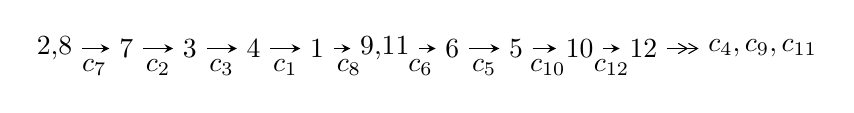
\begin{tikzpicture}[x=23pt, y=7pt]
	% node
	\node (A0) at (-1/8, 0) {2,8};
	\node (A1) at (1, 0) {7};
	\node (A2) at (2, 0) {3};
	\node (A3) at (3, 0) {4};
	\node (A4) at (4, 0) {1};
	\node (A5) at (81/16, 0) {9,11};
	\node (A6) at (49/8, 0) {6};
	\node (A7) at (57/8, 0) {5};
	\node (A8) at (65/8, 0) {10};
	\node (A9) at (73/8, 0) {12};
	\node (C1) at (1/2, -1) {$c_{7}$};
	\node (C2) at (3/2, -1) {$c_{2}$};
	\node (C3) at (5/2, -1) {$c_{3}$};
	\node (C4) at (7/2, -1) {$c_{1}$};
	\node (C5) at (9/2, -1) {$c_{8}$};
	\node (C6) at (45/8, -1) {$c_{6}$};
	\node (C7) at (53/8, -1) {$c_{5}$};
	\node (C8) at (61/8, -1) {$c_{10}$};
	\node (C9) at (69/8, -1) {$c_{12}$};
	\node (A10) at (11, 0) {$c_{4},c_{9},c_{11}$};

	% edge
	\draw[->,>=stealth]	
	(A0) edge (A1) (A1) edge (A2) (A2) edge (A3) (A3) edge (A4) (A4) edge (A5) (A5) edge (A6) (A6) edge (A7) (A7) edge (A8) (A8) edge (A9) ;
	\draw[->>,>={angle 60}]	
	(A9) edge (A10);
\end{tikzpicture} \\ 

\end{tabular} \\

\footnotetext{
The image of knot diagram is generated by the software ``\textbf{Draw programme}" developed by Andrew Bartholomew(\url{http://www.layer8.co.uk/maths/draw/index.htm\#Running-draw}), where we modified some parts for our purpose(\url{https://github.com/CATsTAILs/LinksPainter}).
}\phantom \\ \newline 
\centering \textbf{Ideals for irreducible components\footnotemark of $X_{\text{par}}$} 
 
\begin{align*}
I^u_{1}&=\langle 
3 u^{30}-13 u^{29}+\cdots+2 b-2,\;-7 u^{30}+37 u^{29}+\cdots+4 a-40,\;u^{31}-5 u^{30}+\cdots+26 u-4\rangle \\
I^u_{2}&=\langle 
u^{18}- u^{17}+\cdots+b-2,\;u^{18}+2 u^{17}+\cdots+a+1,\\
\phantom{I^u_{2}}&\phantom{= \langle  }u^{19}+5 u^{17}+13 u^{15}+20 u^{13}+20 u^{11}+13 u^9+u^8+7 u^7+2 u^6+4 u^5+3 u^4+2 u^3+2 u^2+1\rangle \\
I^u_{3}&=\langle 
758 a^3 u^3-3539 u^3 a^2+\cdots+1193 a-9295,\\
\phantom{I^u_{3}}&\phantom{= \langle  }a^3 u^3+a^3 u^2-2 u^3 a^2+a^4+a^3 u- a^2 u^2- a^3+a^2 u-2 u^2 a+u^3- a^2+3 a u+9 u^2+3 a-7 u+2,\\
\phantom{I^u_{3}}&\phantom{= \langle  }u^4+u^2- u+1\rangle \\
I^u_{4}&=\langle 
-18352 u^5 a^3+13327 u^5 a^2+\cdots+704 a-29929,\;u^5 a^2+u^5 a+\cdots+a^4+a^3,\\
\phantom{I^u_{4}}&\phantom{= \langle  }u^6+u^5+2 u^4+2 u^3+2 u^2+2 u+1\rangle \\
\\
\end{align*}
\raggedright * 4 irreducible components of $\dim_{\mathbb{C}}=0$, with total 90 representations.\\
\footnotetext{All coefficients of polynomials are rational numbers. But the coefficients are sometimes approximated in decimal forms when there is not enough margin.}
\newpage
\renewcommand{\arraystretch}{1}
\centering \section*{I. $I^u_{1}= \langle 3 u^{30}-13 u^{29}+\cdots+2 b-2,\;-7 u^{30}+37 u^{29}+\cdots+4 a-40,\;u^{31}-5 u^{30}+\cdots+26 u-4 \rangle$}
\flushleft \textbf{(i) Arc colorings}\\
\begin{tabular}{m{7pt} m{180pt} m{7pt} m{180pt} }
\flushright $a_{2}=$&$\begin{pmatrix}0\\u\end{pmatrix}$ \\
\flushright $a_{8}=$&$\begin{pmatrix}1\\0\end{pmatrix}$ \\
\flushright $a_{7}=$&$\begin{pmatrix}1\\u^2\end{pmatrix}$ \\
\flushright $a_{3}=$&$\begin{pmatrix}u\\u^3+u\end{pmatrix}$ \\
\flushright $a_{4}=$&$\begin{pmatrix}- u^3\\u^3+u\end{pmatrix}$ \\
\flushright $a_{1}=$&$\begin{pmatrix}u^3\\u^5+u^3+u\end{pmatrix}$ \\
\flushright $a_{9}=$&$\begin{pmatrix}u^8+u^6+u^4+1\\u^{10}+2 u^8+3 u^6+2 u^4+u^2\end{pmatrix}$ \\
\flushright $a_{11}=$&$\begin{pmatrix}\frac{7}{4} u^{30}-\frac{37}{4} u^{29}+\cdots-\frac{223}{4} u+10\\-\frac{3}{2} u^{30}+\frac{13}{2} u^{29}+\cdots+\frac{9}{2} u+1\end{pmatrix}$ \\
\flushright $a_{6}=$&$\begin{pmatrix}-\frac{1}{2} u^{30}+\frac{1}{2} u^{28}+\cdots-22 u+\frac{9}{2}\\-\frac{5}{2} u^{30}+\frac{25}{2} u^{29}+\cdots+\frac{139}{2} u-12\end{pmatrix}$ \\
\flushright $a_{5}=$&$\begin{pmatrix}\frac{3}{2} u^{30}-8 u^{29}+\cdots-48 u+\frac{17}{2}\\-\frac{1}{2} u^{30}+\frac{5}{2} u^{29}+\cdots+\frac{21}{2} u-2\end{pmatrix}$ \\
\flushright $a_{10}=$&$\begin{pmatrix}\frac{11}{4} u^{30}-\frac{49}{4} u^{29}+\cdots-\frac{223}{4} u+10\\-\frac{5}{2} u^{30}+\frac{19}{2} u^{29}+\cdots+\frac{29}{2} u-1\end{pmatrix}$ \\
\flushright $a_{12}=$&$\begin{pmatrix}\frac{1}{2} u^{30}-5 u^{29}+\cdots-48 u+\frac{17}{2}\\-\frac{1}{2} u^{30}+\frac{7}{2} u^{29}+\cdots-\frac{3}{2} u+2\end{pmatrix}$\\&\end{tabular}
\flushleft \textbf{(ii) Obstruction class $= -1$}\\~\\
\flushleft \textbf{(iii) Cusp Shapes $= -3 u^{30}+11 u^{29}-40 u^{28}+89 u^{27}-194 u^{26}+336 u^{25}-572 u^{24}+853 u^{23}-1224 u^{22}+1607 u^{21}-2012 u^{20}+2378 u^{19}-2693 u^{18}+2898 u^{17}-3000 u^{16}+2942 u^{15}-2813 u^{14}+2557 u^{13}-2256 u^{12}+1890 u^{11}-1511 u^{10}+1161 u^9-859 u^8+595 u^7-400 u^6+233 u^5-122 u^4+58 u^3-13 u^2+6 u-14$}\\~\\
\newpage\renewcommand{\arraystretch}{1}
\flushleft \textbf{(iv) u-Polynomials at the component}\newline \\
\begin{tabular}{m{50pt}|m{274pt}}
Crossings & \hspace{64pt}u-Polynomials at each crossing \\
\hline $$\begin{aligned}c_{1}\end{aligned}$$&$\begin{aligned}
&u^{31}+15 u^{30}+\cdots+12 u-16
\end{aligned}$\\
\hline $$\begin{aligned}c_{2},c_{7}\end{aligned}$$&$\begin{aligned}
&u^{31}+5 u^{30}+\cdots+26 u+4
\end{aligned}$\\
\hline $$\begin{aligned}c_{3}\end{aligned}$$&$\begin{aligned}
&u^{31}-5 u^{30}+\cdots-240 u+32
\end{aligned}$\\
\hline $$\begin{aligned}c_{4},c_{6},c_{10}\\c_{11}\end{aligned}$$&$\begin{aligned}
&u^{31}+7 u^{29}+\cdots+3 u+1
\end{aligned}$\\
\hline $$\begin{aligned}c_{5},c_{9}\end{aligned}$$&$\begin{aligned}
&u^{31}+u^{30}+\cdots+4 u+1
\end{aligned}$\\
\hline $$\begin{aligned}c_{8}\end{aligned}$$&$\begin{aligned}
&u^{31}+25 u^{30}+\cdots+101226 u+9028
\end{aligned}$\\
\hline $$\begin{aligned}c_{12}\end{aligned}$$&$\begin{aligned}
&u^{31}-24 u^{30}+\cdots-9728 u+1024
\end{aligned}$\\
\hline
\end{tabular}\\~\\
\newpage\renewcommand{\arraystretch}{1}
\flushleft \textbf{(v) Riley Polynomials at the component}\newline \\
\begin{tabular}{m{50pt}|m{274pt}}
Crossings & \hspace{64pt}Riley Polynomials at each crossing \\
\hline $$\begin{aligned}c_{1}\end{aligned}$$&$\begin{aligned}
&y^{31}+3 y^{30}+\cdots+5360 y-256
\end{aligned}$\\
\hline $$\begin{aligned}c_{2},c_{7}\end{aligned}$$&$\begin{aligned}
&y^{31}+15 y^{30}+\cdots+12 y-16
\end{aligned}$\\
\hline $$\begin{aligned}c_{3}\end{aligned}$$&$\begin{aligned}
&y^{31}-9 y^{30}+\cdots+29696 y-1024
\end{aligned}$\\
\hline $$\begin{aligned}c_{4},c_{6},c_{10}\\c_{11}\end{aligned}$$&$\begin{aligned}
&y^{31}+14 y^{30}+\cdots-11 y-1
\end{aligned}$\\
\hline $$\begin{aligned}c_{5},c_{9}\end{aligned}$$&$\begin{aligned}
&y^{31}-49 y^{30}+\cdots+50 y-1
\end{aligned}$\\
\hline $$\begin{aligned}c_{8}\end{aligned}$$&$\begin{aligned}
&y^{31}+3 y^{30}+\cdots-146312468 y-81504784
\end{aligned}$\\
\hline $$\begin{aligned}c_{12}\end{aligned}$$&$\begin{aligned}
&y^{31}-18 y^{30}+\cdots+4980736 y-1048576
\end{aligned}$\\
\hline
\end{tabular}\\~\\
\newpage\flushleft \textbf{(vi) Complex Volumes and Cusp Shapes}
$$\begin{array}{c|c|c}  
\text{Solutions to }I^u_{1}& \I (\text{vol} + \sqrt{-1}CS) & \text{Cusp shape}\\
 \hline 
\begin{aligned}
u &= -0.721636 + 0.688504 I \\
a &= \phantom{-}0.652136 - 0.856774 I \\
b &= -0.153998 + 0.558335 I\end{aligned}
 & \phantom{-}0.12057 - 7.84511 I & -4.92980 + 6.31603 I \\ \hline\begin{aligned}
u &= -0.721636 - 0.688504 I \\
a &= \phantom{-}0.652136 + 0.856774 I \\
b &= -0.153998 - 0.558335 I\end{aligned}
 & \phantom{-}0.12057 + 7.84511 I & -4.92980 - 6.31603 I \\ \hline\begin{aligned}
u &= \phantom{-}0.107386 + 1.053710 I \\
a &= \phantom{-}1.161140 + 0.418626 I \\
b &= -0.848962 + 0.418880 I\end{aligned}
 & -1.06007 - 1.48672 I & -11.73110 + 4.30166 I \\ \hline\begin{aligned}
u &= \phantom{-}0.107386 - 1.053710 I \\
a &= \phantom{-}1.161140 - 0.418626 I \\
b &= -0.848962 - 0.418880 I\end{aligned}
 & -1.06007 + 1.48672 I & -11.73110 - 4.30166 I \\ \hline\begin{aligned}
u &= -0.747524 + 0.519989 I \\
a &= -0.367732 + 0.710748 I \\
b &= \phantom{-}0.063240 - 0.394635 I\end{aligned}
 & \phantom{-}4.39870 - 0.57100 I & -5.18268 + 2.58205 I \\ \hline\begin{aligned}
u &= -0.747524 - 0.519989 I \\
a &= -0.367732 - 0.710748 I \\
b &= \phantom{-}0.063240 + 0.394635 I\end{aligned}
 & \phantom{-}4.39870 + 0.57100 I & -5.18268 - 2.58205 I \\ \hline\begin{aligned}
u &= -0.228069 + 0.871292 I \\
a &= \phantom{-}0.493234 - 0.013294 I \\
b &= -0.220969 + 0.195636 I\end{aligned}
 & -0.647219 - 1.174890 I & -7.74715 + 5.33716 I \\ \hline\begin{aligned}
u &= -0.228069 - 0.871292 I \\
a &= \phantom{-}0.493234 + 0.013294 I \\
b &= -0.220969 - 0.195636 I\end{aligned}
 & -0.647219 + 1.174890 I & -7.74715 - 5.33716 I \\ \hline\begin{aligned}
u &= \phantom{-}0.826592 + 0.330880 I \\
a &= \phantom{-}0.611177 - 0.577058 I \\
b &= \phantom{-}1.51649 + 1.30911 I\end{aligned}
 & -1.86480 - 10.61960 I & -6.01076 + 5.40369 I \\ \hline\begin{aligned}
u &= \phantom{-}0.826592 - 0.330880 I \\
a &= \phantom{-}0.611177 + 0.577058 I \\
b &= \phantom{-}1.51649 - 1.30911 I\end{aligned}
 & -1.86480 + 10.61960 I & -6.01076 - 5.40369 I\\
 \hline 
 \end{array}$$\newpage$$\begin{array}{c|c|c}  
\text{Solutions to }I^u_{1}& \I (\text{vol} + \sqrt{-1}CS) & \text{Cusp shape}\\
 \hline 
\begin{aligned}
u &= \phantom{-}0.771083 + 0.435830 I \\
a &= -0.445507 + 0.696759 I \\
b &= -1.22832 - 0.83980 I\end{aligned}
 & \phantom{-}3.95523 - 3.38934 I & -6.35399 + 4.30144 I \\ \hline\begin{aligned}
u &= \phantom{-}0.771083 - 0.435830 I \\
a &= -0.445507 - 0.696759 I \\
b &= -1.22832 + 0.83980 I\end{aligned}
 & \phantom{-}3.95523 + 3.38934 I & -6.35399 - 4.30144 I \\ \hline\begin{aligned}
u &= -0.659178 + 0.906469 I \\
a &= \phantom{-}0.847117 + 0.308890 I \\
b &= -0.532248 + 0.049305 I\end{aligned}
 & -0.52577 + 2.60216 I & -5.79015 - 0.92756 I \\ \hline\begin{aligned}
u &= -0.659178 - 0.906469 I \\
a &= \phantom{-}0.847117 - 0.308890 I \\
b &= -0.532248 - 0.049305 I\end{aligned}
 & -0.52577 - 2.60216 I & -5.79015 + 0.92756 I \\ \hline\begin{aligned}
u &= \phantom{-}0.431568 + 1.070840 I \\
a &= -1.72983 - 0.61820 I \\
b &= \phantom{-}1.51123 - 0.88116 I\end{aligned}
 & -3.48253 + 3.49821 I & -13.1203 - 5.5567 I \\ \hline\begin{aligned}
u &= \phantom{-}0.431568 - 1.070840 I \\
a &= -1.72983 + 0.61820 I \\
b &= \phantom{-}1.51123 + 0.88116 I\end{aligned}
 & -3.48253 - 3.49821 I & -13.1203 + 5.5567 I \\ \hline\begin{aligned}
u &= \phantom{-}0.831503 + 0.123089 I \\
a &= \phantom{-}0.072492 + 0.269764 I \\
b &= -0.554560 + 0.979079 I\end{aligned}
 & -4.92001 + 1.57506 I & -6.24630 - 4.36146 I \\ \hline\begin{aligned}
u &= \phantom{-}0.831503 - 0.123089 I \\
a &= \phantom{-}0.072492 - 0.269764 I \\
b &= -0.554560 - 0.979079 I\end{aligned}
 & -4.92001 - 1.57506 I & -6.24630 + 4.36146 I \\ \hline\begin{aligned}
u &= \phantom{-}0.210275 + 1.194020 I \\
a &= -1.29566 - 1.42704 I \\
b &= \phantom{-}1.62781 + 0.12223 I\end{aligned}
 & -6.84341 - 7.58988 I & -11.74966 + 3.94255 I \\ \hline\begin{aligned}
u &= \phantom{-}0.210275 - 1.194020 I \\
a &= -1.29566 + 1.42704 I \\
b &= \phantom{-}1.62781 - 0.12223 I\end{aligned}
 & -6.84341 + 7.58988 I & -11.74966 - 3.94255 I\\
 \hline 
 \end{array}$$\newpage$$\begin{array}{c|c|c}  
\text{Solutions to }I^u_{1}& \I (\text{vol} + \sqrt{-1}CS) & \text{Cusp shape}\\
 \hline 
\begin{aligned}
u &= -0.618523 + 1.046160 I \\
a &= -0.569195 - 0.233428 I \\
b &= \phantom{-}0.386901 - 0.028623 I\end{aligned}
 & \phantom{-}2.83735 - 4.61812 I & -7.27766 + 3.11789 I \\ \hline\begin{aligned}
u &= -0.618523 - 1.046160 I \\
a &= -0.569195 + 0.233428 I \\
b &= \phantom{-}0.386901 + 0.028623 I\end{aligned}
 & \phantom{-}2.83735 + 4.61812 I & -7.27766 - 3.11789 I \\ \hline\begin{aligned}
u &= \phantom{-}0.601498 + 1.094000 I \\
a &= \phantom{-}1.80478 + 0.82107 I \\
b &= -1.93685 + 0.87675 I\end{aligned}
 & \phantom{-}2.00079 + 8.57439 I & -9.56481 - 9.13529 I \\ \hline\begin{aligned}
u &= \phantom{-}0.601498 - 1.094000 I \\
a &= \phantom{-}1.80478 - 0.82107 I \\
b &= -1.93685 - 0.87675 I\end{aligned}
 & \phantom{-}2.00079 - 8.57439 I & -9.56481 + 9.13529 I \\ \hline\begin{aligned}
u &= \phantom{-}0.372959 + 1.216560 I \\
a &= \phantom{-}1.28688 - 0.66870 I \\
b &= -0.421817 + 1.280630 I\end{aligned}
 & -9.03283 + 5.64879 I & -11.83814 - 7.15330 I \\ \hline\begin{aligned}
u &= \phantom{-}0.372959 - 1.216560 I \\
a &= \phantom{-}1.28688 + 0.66870 I \\
b &= -0.421817 - 1.280630 I\end{aligned}
 & -9.03283 - 5.64879 I & -11.83814 + 7.15330 I \\ \hline\begin{aligned}
u &= \phantom{-}0.587276 + 1.148200 I \\
a &= -2.51290 - 0.46864 I \\
b &= \phantom{-}2.17768 - 1.59943 I\end{aligned}
 & -4.3002 + 15.8732 I & -8.95437 - 9.00468 I \\ \hline\begin{aligned}
u &= \phantom{-}0.587276 - 1.148200 I \\
a &= -2.51290 + 0.46864 I \\
b &= \phantom{-}2.17768 + 1.59943 I\end{aligned}
 & -4.3002 - 15.8732 I & -8.95437 + 9.00468 I \\ \hline\begin{aligned}
u &= \phantom{-}0.501811 + 1.205770 I \\
a &= -0.157189 + 1.192800 I \\
b &= -0.733813 - 0.955023 I\end{aligned}
 & -8.15901 + 3.28278 I & -8.89616 + 2.41825 I \\ \hline\begin{aligned}
u &= \phantom{-}0.501811 - 1.205770 I \\
a &= -0.157189 - 1.192800 I \\
b &= -0.733813 + 0.955023 I\end{aligned}
 & -8.15901 - 3.28278 I & -8.89616 - 2.41825 I\\
 \hline 
 \end{array}$$\newpage$$\begin{array}{c|c|c}  
\text{Solutions to }I^u_{1}& \I (\text{vol} + \sqrt{-1}CS) & \text{Cusp shape}\\
 \hline 
\begin{aligned}
u &= \phantom{-}0.465958\phantom{ +0.000000I} \\
a &= \phantom{-}0.798102\phantom{ +0.000000I} \\
b &= \phantom{-}0.696353\phantom{ +0.000000I}\end{aligned}
 & -0.881419\phantom{ +0.000000I} & -11.2140\phantom{ +0.000000I}\\
 \hline 
 \end{array}$$\newpage\newpage\renewcommand{\arraystretch}{1}
\centering \section*{II. $I^u_{2}= \langle u^{18}- u^{17}+\cdots+b-2,\;u^{18}+2 u^{17}+\cdots+a+1,\;u^{19}+5 u^{17}+\cdots+2 u^2+1 \rangle$}
\flushleft \textbf{(i) Arc colorings}\\
\begin{tabular}{m{7pt} m{180pt} m{7pt} m{180pt} }
\flushright $a_{2}=$&$\begin{pmatrix}0\\u\end{pmatrix}$ \\
\flushright $a_{8}=$&$\begin{pmatrix}1\\0\end{pmatrix}$ \\
\flushright $a_{7}=$&$\begin{pmatrix}1\\u^2\end{pmatrix}$ \\
\flushright $a_{3}=$&$\begin{pmatrix}u\\u^3+u\end{pmatrix}$ \\
\flushright $a_{4}=$&$\begin{pmatrix}- u^3\\u^3+u\end{pmatrix}$ \\
\flushright $a_{1}=$&$\begin{pmatrix}u^3\\u^5+u^3+u\end{pmatrix}$ \\
\flushright $a_{9}=$&$\begin{pmatrix}u^8+u^6+u^4+1\\u^{10}+2 u^8+3 u^6+2 u^4+u^2\end{pmatrix}$ \\
\flushright $a_{11}=$&$\begin{pmatrix}- u^{18}-2 u^{17}+\cdots-3 u-1\\- u^{18}+u^{17}+\cdots+u+2\end{pmatrix}$ \\
\flushright $a_{6}=$&$\begin{pmatrix}u^{17}+5 u^{15}+\cdots+u+2\\u^{18}+5 u^{16}+\cdots+u^3-1\end{pmatrix}$ \\
\flushright $a_{5}=$&$\begin{pmatrix}2 u^{17}+9 u^{15}+\cdots+u+2\\u^{18}+5 u^{16}+\cdots+u-1\end{pmatrix}$ \\
\flushright $a_{10}=$&$\begin{pmatrix}-2 u^{17}- u^{16}+\cdots-2 u-1\\- u^{18}+u^{17}+\cdots+2 u^2+2\end{pmatrix}$ \\
\flushright $a_{12}=$&$\begin{pmatrix}-3 u^{18}-2 u^{17}+\cdots-6 u-2\\- u^{18}+u^{17}+\cdots+2 u+3\end{pmatrix}$\\&\end{tabular}
\flushleft \textbf{(ii) Obstruction class $= 1$}\\~\\
\flushleft \textbf{(iii) Cusp Shapes $= -2 u^{17}-10 u^{15}+4 u^{14}-24 u^{13}+12 u^{12}-34 u^{11}+17 u^{10}-30 u^9+6 u^8-18 u^7-7 u^6-7 u^5-6 u^4+u^3+u^2+u-10$}\\~\\
\newpage\renewcommand{\arraystretch}{1}
\flushleft \textbf{(iv) u-Polynomials at the component}\newline \\
\begin{tabular}{m{50pt}|m{274pt}}
Crossings & \hspace{64pt}u-Polynomials at each crossing \\
\hline $$\begin{aligned}c_{1}\end{aligned}$$&$\begin{aligned}
&u^{19}-10 u^{18}+\cdots-4 u+1
\end{aligned}$\\
\hline $$\begin{aligned}c_{2}\end{aligned}$$&$\begin{aligned}
&u^{19}+5 u^{17}+\cdots-2 u^2-1
\end{aligned}$\\
\hline $$\begin{aligned}c_{3}\end{aligned}$$&$\begin{aligned}
&u^{19}-3 u^{17}+\cdots+3 u-2
\end{aligned}$\\
\hline $$\begin{aligned}c_{4},c_{11}\end{aligned}$$&$\begin{aligned}
&u^{19}+6 u^{17}+\cdots- u+1
\end{aligned}$\\
\hline $$\begin{aligned}c_{5},c_{9}\end{aligned}$$&$\begin{aligned}
&u^{19}- u^{18}+\cdots+6 u^2+1
\end{aligned}$\\
\hline $$\begin{aligned}c_{6},c_{10}\end{aligned}$$&$\begin{aligned}
&u^{19}+6 u^{17}+\cdots- u-1
\end{aligned}$\\
\hline $$\begin{aligned}c_{7}\end{aligned}$$&$\begin{aligned}
&u^{19}+5 u^{17}+\cdots+2 u^2+1
\end{aligned}$\\
\hline $$\begin{aligned}c_{8}\end{aligned}$$&$\begin{aligned}
&u^{19}+u^{17}+\cdots+3 u^2+1
\end{aligned}$\\
\hline $$\begin{aligned}c_{12}\end{aligned}$$&$\begin{aligned}
&u^{19}+7 u^{18}+\cdots+3 u+2
\end{aligned}$\\
\hline
\end{tabular}\\~\\
\newpage\renewcommand{\arraystretch}{1}
\flushleft \textbf{(v) Riley Polynomials at the component}\newline \\
\begin{tabular}{m{50pt}|m{274pt}}
Crossings & \hspace{64pt}Riley Polynomials at each crossing \\
\hline $$\begin{aligned}c_{1}\end{aligned}$$&$\begin{aligned}
&y^{19}+2 y^{18}+\cdots-4 y-1
\end{aligned}$\\
\hline $$\begin{aligned}c_{2},c_{7}\end{aligned}$$&$\begin{aligned}
&y^{19}+10 y^{18}+\cdots-4 y-1
\end{aligned}$\\
\hline $$\begin{aligned}c_{3}\end{aligned}$$&$\begin{aligned}
&y^{19}-6 y^{18}+\cdots+5 y-4
\end{aligned}$\\
\hline $$\begin{aligned}c_{4},c_{6},c_{10}\\c_{11}\end{aligned}$$&$\begin{aligned}
&y^{19}+12 y^{18}+\cdots+7 y-1
\end{aligned}$\\
\hline $$\begin{aligned}c_{5},c_{9}\end{aligned}$$&$\begin{aligned}
&y^{19}-7 y^{18}+\cdots-12 y-1
\end{aligned}$\\
\hline $$\begin{aligned}c_{8}\end{aligned}$$&$\begin{aligned}
&y^{19}+2 y^{18}+\cdots-6 y-1
\end{aligned}$\\
\hline $$\begin{aligned}c_{12}\end{aligned}$$&$\begin{aligned}
&y^{19}-15 y^{18}+\cdots-35 y-4
\end{aligned}$\\
\hline
\end{tabular}\\~\\
\newpage\flushleft \textbf{(vi) Complex Volumes and Cusp Shapes}
$$\begin{array}{c|c|c}  
\text{Solutions to }I^u_{2}& \I (\text{vol} + \sqrt{-1}CS) & \text{Cusp shape}\\
 \hline 
\begin{aligned}
u &= -0.342966 + 0.928812 I \\
a &= \phantom{-}1.348510 + 0.263101 I \\
b &= -0.760930 + 0.339185 I\end{aligned}
 & \phantom{-}2.81022 - 1.37153 I & -9.77927 + 0.03000 I \\ \hline\begin{aligned}
u &= -0.342966 - 0.928812 I \\
a &= \phantom{-}1.348510 - 0.263101 I \\
b &= -0.760930 - 0.339185 I\end{aligned}
 & \phantom{-}2.81022 + 1.37153 I & -9.77927 - 0.03000 I \\ \hline\begin{aligned}
u &= \phantom{-}0.462820 + 1.013630 I \\
a &= -2.71881 - 1.75930 I \\
b &= \phantom{-}2.96409 - 1.05294 I\end{aligned}
 & -5.17143 + 3.04865 I & -17.3001 - 5.4133 I \\ \hline\begin{aligned}
u &= \phantom{-}0.462820 - 1.013630 I \\
a &= -2.71881 + 1.75930 I \\
b &= \phantom{-}2.96409 + 1.05294 I\end{aligned}
 & -5.17143 - 3.04865 I & -17.3001 + 5.4133 I \\ \hline\begin{aligned}
u &= \phantom{-}0.233225 + 1.122880 I \\
a &= \phantom{-}0.57215 + 1.46143 I \\
b &= -1.222460 - 0.507809 I\end{aligned}
 & \phantom{-}0.773516 - 0.146851 I & -4.77195 + 0.70902 I \\ \hline\begin{aligned}
u &= \phantom{-}0.233225 - 1.122880 I \\
a &= \phantom{-}0.57215 - 1.46143 I \\
b &= -1.222460 + 0.507809 I\end{aligned}
 & \phantom{-}0.773516 + 0.146851 I & -4.77195 - 0.70902 I \\ \hline\begin{aligned}
u &= -0.666278 + 0.525489 I \\
a &= -0.803308 + 0.905672 I \\
b &= \phantom{-}0.208916 - 0.549594 I\end{aligned}
 & \phantom{-}6.17150 - 0.46362 I & \phantom{-}0.865849 + 0.093263 I \\ \hline\begin{aligned}
u &= -0.666278 - 0.525489 I \\
a &= -0.803308 - 0.905672 I \\
b &= \phantom{-}0.208916 + 0.549594 I\end{aligned}
 & \phantom{-}6.17150 + 0.46362 I & \phantom{-}0.865849 - 0.093263 I \\ \hline\begin{aligned}
u &= \phantom{-}0.755679 + 0.375560 I \\
a &= -0.759994 + 0.411460 I \\
b &= -0.93480 - 1.33254 I\end{aligned}
 & \phantom{-}5.35455 - 2.68854 I & \phantom{-}0.27590 + 1.63116 I \\ \hline\begin{aligned}
u &= \phantom{-}0.755679 - 0.375560 I \\
a &= -0.759994 - 0.411460 I \\
b &= -0.93480 + 1.33254 I\end{aligned}
 & \phantom{-}5.35455 + 2.68854 I & \phantom{-}0.27590 - 1.63116 I\\
 \hline 
 \end{array}$$\newpage$$\begin{array}{c|c|c}  
\text{Solutions to }I^u_{2}& \I (\text{vol} + \sqrt{-1}CS) & \text{Cusp shape}\\
 \hline 
\begin{aligned}
u &= -0.572364 + 1.036080 I \\
a &= -0.875217 - 0.298710 I \\
b &= \phantom{-}0.574390 - 0.089490 I\end{aligned}
 & \phantom{-}4.65158 - 4.35826 I & -3.03168 + 5.37971 I \\ \hline\begin{aligned}
u &= -0.572364 - 1.036080 I \\
a &= -0.875217 + 0.298710 I \\
b &= \phantom{-}0.574390 + 0.089490 I\end{aligned}
 & \phantom{-}4.65158 + 4.35826 I & -3.03168 - 5.37971 I \\ \hline\begin{aligned}
u &= \phantom{-}0.583300 + 1.114080 I \\
a &= \phantom{-}2.02438 + 0.07803 I \\
b &= -1.48959 + 1.53903 I\end{aligned}
 & \phantom{-}3.18311 + 7.76425 I & -3.26242 - 5.87229 I \\ \hline\begin{aligned}
u &= \phantom{-}0.583300 - 1.114080 I \\
a &= \phantom{-}2.02438 - 0.07803 I \\
b &= -1.48959 - 1.53903 I\end{aligned}
 & \phantom{-}3.18311 - 7.76425 I & -3.26242 + 5.87229 I \\ \hline\begin{aligned}
u &= -0.458473 + 1.178850 I \\
a &= -0.111178 + 0.351572 I \\
b &= -0.052777 - 0.243038 I\end{aligned}
 & -8.21489 - 4.24741 I & -10.19096 + 5.10189 I \\ \hline\begin{aligned}
u &= -0.458473 - 1.178850 I \\
a &= -0.111178 - 0.351572 I \\
b &= -0.052777 + 0.243038 I\end{aligned}
 & -8.21489 + 4.24741 I & -10.19096 - 5.10189 I \\ \hline\begin{aligned}
u &= \phantom{-}0.351995 + 0.609402 I \\
a &= \phantom{-}0.67301 - 2.19679 I \\
b &= \phantom{-}1.56998 + 0.91609 I\end{aligned}
 & -3.79826 + 0.59510 I & -11.16480 + 2.33336 I \\ \hline\begin{aligned}
u &= \phantom{-}0.351995 - 0.609402 I \\
a &= \phantom{-}0.67301 + 2.19679 I \\
b &= \phantom{-}1.56998 - 0.91609 I\end{aligned}
 & -3.79826 - 0.59510 I & -11.16480 - 2.33336 I \\ \hline\begin{aligned}
u &= -0.693876\phantom{ +0.000000I} \\
a &= -0.699080\phantom{ +0.000000I} \\
b &= \phantom{-}0.286370\phantom{ +0.000000I}\end{aligned}
 & -4.94005\phantom{ +0.000000I} & -7.28110\phantom{ +0.000000I}\\
 \hline 
 \end{array}$$\newpage\newpage\renewcommand{\arraystretch}{1}
\centering \section*{III. $I^u_{3}= \langle 758 a^3 u^3-3539 u^3 a^2+\cdots+1193 a-9295,\;a^3 u^3-2 u^3 a^2+\cdots+3 a+2,\;u^4+u^2- u+1 \rangle$}
\flushleft \textbf{(i) Arc colorings}\\
\begin{tabular}{m{7pt} m{180pt} m{7pt} m{180pt} }
\flushright $a_{2}=$&$\begin{pmatrix}0\\u\end{pmatrix}$ \\
\flushright $a_{8}=$&$\begin{pmatrix}1\\0\end{pmatrix}$ \\
\flushright $a_{7}=$&$\begin{pmatrix}1\\u^2\end{pmatrix}$ \\
\flushright $a_{3}=$&$\begin{pmatrix}u\\u^3+u\end{pmatrix}$ \\
\flushright $a_{4}=$&$\begin{pmatrix}- u^3\\u^3+u\end{pmatrix}$ \\
\flushright $a_{1}=$&$\begin{pmatrix}u^3\\u^2\end{pmatrix}$ \\
\flushright $a_{9}=$&$\begin{pmatrix}- u^3+u^2- u+1\\- u^2+u-1\end{pmatrix}$ \\
\flushright $a_{11}=$&$\begin{pmatrix}a\\-0.0877721 a^{3} u^{3}+0.409796 a^{2} u^{3}+\cdots-0.138143 a+1.07631\end{pmatrix}$ \\
\flushright $a_{6}=$&$\begin{pmatrix}-0.0211904 a^{3} u^{3}+0.0128532 a^{2} u^{3}+\cdots+0.183997 a-0.0683187\\0.0507179 a^{3} u^{3}-0.325845 a^{2} u^{3}+\cdots-0.178092 a-0.754516\end{pmatrix}$ \\
\flushright $a_{5}=$&$\begin{pmatrix}-0.0620658 a^{3} u^{3}+0.234368 a^{2} u^{3}+\cdots+0.364057 a-0.254748\\0.189787 a^{3} u^{3}-0.0823298 a^{2} u^{3}+\cdots-0.232631 a-1.50834\end{pmatrix}$ \\
\flushright $a_{10}=$&$\begin{pmatrix}-0.100741 a^{3} u^{3}-0.123321 a^{2} u^{3}+\cdots+0.788675 a+0.351436\\-0.0507179 a^{3} u^{3}+0.575845 a^{2} u^{3}+\cdots+0.428092 a+1.50452\end{pmatrix}$ \\
\flushright $a_{12}=$&$\begin{pmatrix}-0.0211904 a^{3} u^{3}+0.0128532 a^{2} u^{3}+\cdots+0.183997 a-0.0683187\\0.0100741 a^{3} u^{3}+0.387332 a^{2} u^{3}+\cdots-0.103868 a+2.58986\end{pmatrix}$\\&\end{tabular}
\flushleft \textbf{(ii) Obstruction class $= -1$}\\~\\
\flushleft \textbf{(iii) Cusp Shapes $= -4 u^3-4 u^2-6$}\\~\\
\newpage\renewcommand{\arraystretch}{1}
\flushleft \textbf{(iv) u-Polynomials at the component}\newline \\
\begin{tabular}{m{50pt}|m{274pt}}
Crossings & \hspace{64pt}u-Polynomials at each crossing \\
\hline $$\begin{aligned}c_{1}\end{aligned}$$&$\begin{aligned}
&(u^4+2 u^3+3 u^2+u+1)^4
\end{aligned}$\\
\hline $$\begin{aligned}c_{2},c_{7}\end{aligned}$$&$\begin{aligned}
&(u^4+u^2+u+1)^4
\end{aligned}$\\
\hline $$\begin{aligned}c_{3}\end{aligned}$$&$\begin{aligned}
&(u^4+3 u^3+4 u^2+3 u+2)^4
\end{aligned}$\\
\hline $$\begin{aligned}c_{4},c_{6},c_{10}\\c_{11}\end{aligned}$$&$\begin{aligned}
&u^{16}+3 u^{14}+\cdots+4 u+19
\end{aligned}$\\
\hline $$\begin{aligned}c_{5},c_{9}\end{aligned}$$&$\begin{aligned}
&u^{16}-5 u^{14}+\cdots-26 u+31
\end{aligned}$\\
\hline $$\begin{aligned}c_{8}\end{aligned}$$&$\begin{aligned}
&(u^4-2 u^3+3 u^2- u+1)^4
\end{aligned}$\\
\hline $$\begin{aligned}c_{12}\end{aligned}$$&$\begin{aligned}
&(u^2+u-1)^8
\end{aligned}$\\
\hline
\end{tabular}\\~\\
\newpage\renewcommand{\arraystretch}{1}
\flushleft \textbf{(v) Riley Polynomials at the component}\newline \\
\begin{tabular}{m{50pt}|m{274pt}}
Crossings & \hspace{64pt}Riley Polynomials at each crossing \\
\hline $$\begin{aligned}c_{1},c_{8}\end{aligned}$$&$\begin{aligned}
&(y^4+2 y^3+7 y^2+5 y+1)^4
\end{aligned}$\\
\hline $$\begin{aligned}c_{2},c_{7}\end{aligned}$$&$\begin{aligned}
&(y^4+2 y^3+3 y^2+y+1)^4
\end{aligned}$\\
\hline $$\begin{aligned}c_{3}\end{aligned}$$&$\begin{aligned}
&(y^4- y^3+2 y^2+7 y+4)^4
\end{aligned}$\\
\hline $$\begin{aligned}c_{4},c_{6},c_{10}\\c_{11}\end{aligned}$$&$\begin{aligned}
&y^{16}+6 y^{15}+\cdots+1428 y+361
\end{aligned}$\\
\hline $$\begin{aligned}c_{5},c_{9}\end{aligned}$$&$\begin{aligned}
&y^{16}-10 y^{15}+\cdots-5760 y+961
\end{aligned}$\\
\hline $$\begin{aligned}c_{12}\end{aligned}$$&$\begin{aligned}
&(y^2-3 y+1)^8
\end{aligned}$\\
\hline
\end{tabular}\\~\\
\newpage\flushleft \textbf{(vi) Complex Volumes and Cusp Shapes}
$$\begin{array}{c|c|c}  
\text{Solutions to }I^u_{3}& \I (\text{vol} + \sqrt{-1}CS) & \text{Cusp shape}\\
 \hline 
\begin{aligned}
u &= \phantom{-}0.547424 + 0.585652 I \\
a &= \phantom{-}0.499523 - 0.414695 I \\
b &= \phantom{-}1.49449 + 0.67486 I\end{aligned}
 & -2.96775 + 1.39709 I & -4.22981 - 3.86736 I \\ \hline\begin{aligned}
u &= \phantom{-}0.547424 + 0.585652 I \\
a &= -1.41065 - 0.30491 I \\
b &= -0.139658 + 0.204609 I\end{aligned}
 & \phantom{-}4.92794 + 1.39709 I & -4.22981 - 3.86736 I \\ \hline\begin{aligned}
u &= \phantom{-}0.547424 + 0.585652 I \\
a &= \phantom{-}0.85743 + 1.26440 I \\
b &= -0.789932 - 0.962845 I\end{aligned}
 & \phantom{-}4.92794 + 1.39709 I & -4.22981 - 3.86736 I \\ \hline\begin{aligned}
u &= \phantom{-}0.547424 + 0.585652 I \\
a &= \phantom{-}0.94882 - 2.09729 I \\
b &= \phantom{-}0.93920 + 1.31022 I\end{aligned}
 & -2.96775 + 1.39709 I & -4.22981 - 3.86736 I \\ \hline\begin{aligned}
u &= \phantom{-}0.547424 - 0.585652 I \\
a &= \phantom{-}0.499523 + 0.414695 I \\
b &= \phantom{-}1.49449 - 0.67486 I\end{aligned}
 & -2.96775 - 1.39709 I & -4.22981 + 3.86736 I \\ \hline\begin{aligned}
u &= \phantom{-}0.547424 - 0.585652 I \\
a &= -1.41065 + 0.30491 I \\
b &= -0.139658 - 0.204609 I\end{aligned}
 & \phantom{-}4.92794 - 1.39709 I & -4.22981 + 3.86736 I \\ \hline\begin{aligned}
u &= \phantom{-}0.547424 - 0.585652 I \\
a &= \phantom{-}0.85743 - 1.26440 I \\
b &= -0.789932 + 0.962845 I\end{aligned}
 & \phantom{-}4.92794 - 1.39709 I & -4.22981 + 3.86736 I \\ \hline\begin{aligned}
u &= \phantom{-}0.547424 - 0.585652 I \\
a &= \phantom{-}0.94882 + 2.09729 I \\
b &= \phantom{-}0.93920 - 1.31022 I\end{aligned}
 & -2.96775 - 1.39709 I & -4.22981 + 3.86736 I \\ \hline\begin{aligned}
u &= -0.547424 + 1.120870 I \\
a &= \phantom{-}1.98981 - 0.07512 I \\
b &= -1.28422 - 1.69317 I\end{aligned}
 & \phantom{-}1.32281 - 7.64338 I & -9.77019 + 6.51087 I \\ \hline\begin{aligned}
u &= -0.547424 + 1.120870 I \\
a &= -0.79640 + 1.83226 I \\
b &= \phantom{-}1.57066 - 0.08141 I\end{aligned}
 & -6.57287 - 7.64338 I & -9.77019 + 6.51087 I\\
 \hline 
 \end{array}$$\newpage$$\begin{array}{c|c|c}  
\text{Solutions to }I^u_{3}& \I (\text{vol} + \sqrt{-1}CS) & \text{Cusp shape}\\
 \hline 
\begin{aligned}
u &= -0.547424 + 1.120870 I \\
a &= \phantom{-}1.77511 - 1.01217 I \\
b &= -2.38632 - 0.09060 I\end{aligned}
 & -6.57287 - 7.64338 I & -9.77019 + 6.51087 I \\ \hline\begin{aligned}
u &= -0.547424 + 1.120870 I \\
a &= -2.36364 - 0.23813 I \\
b &= \phantom{-}1.59578 + 1.75888 I\end{aligned}
 & \phantom{-}1.32281 - 7.64338 I & -9.77019 + 6.51087 I \\ \hline\begin{aligned}
u &= -0.547424 - 1.120870 I \\
a &= \phantom{-}1.98981 + 0.07512 I \\
b &= -1.28422 + 1.69317 I\end{aligned}
 & \phantom{-}1.32281 + 7.64338 I & -9.77019 - 6.51087 I \\ \hline\begin{aligned}
u &= -0.547424 - 1.120870 I \\
a &= -0.79640 - 1.83226 I \\
b &= \phantom{-}1.57066 + 0.08141 I\end{aligned}
 & -6.57287 + 7.64338 I & -9.77019 - 6.51087 I \\ \hline\begin{aligned}
u &= -0.547424 - 1.120870 I \\
a &= \phantom{-}1.77511 + 1.01217 I \\
b &= -2.38632 + 0.09060 I\end{aligned}
 & -6.57287 + 7.64338 I & -9.77019 - 6.51087 I \\ \hline\begin{aligned}
u &= -0.547424 - 1.120870 I \\
a &= -2.36364 + 0.23813 I \\
b &= \phantom{-}1.59578 - 1.75888 I\end{aligned}
 & \phantom{-}1.32281 + 7.64338 I & -9.77019 - 6.51087 I\\
 \hline 
 \end{array}$$\newpage\newpage\renewcommand{\arraystretch}{1}
\centering \section*{IV. $I^u_{4}= \langle -18352 u^5 a^3+13327 u^5 a^2+\cdots+704 a-29929,\;u^5 a^2+u^5 a+\cdots+a^4+a^3,\;u^6+u^5+2 u^4+2 u^3+2 u^2+2 u+1 \rangle$}
\flushleft \textbf{(i) Arc colorings}\\
\begin{tabular}{m{7pt} m{180pt} m{7pt} m{180pt} }
\flushright $a_{2}=$&$\begin{pmatrix}0\\u\end{pmatrix}$ \\
\flushright $a_{8}=$&$\begin{pmatrix}1\\0\end{pmatrix}$ \\
\flushright $a_{7}=$&$\begin{pmatrix}1\\u^2\end{pmatrix}$ \\
\flushright $a_{3}=$&$\begin{pmatrix}u\\u^3+u\end{pmatrix}$ \\
\flushright $a_{4}=$&$\begin{pmatrix}- u^3\\u^3+u\end{pmatrix}$ \\
\flushright $a_{1}=$&$\begin{pmatrix}u^3\\u^5+u^3+u\end{pmatrix}$ \\
\flushright $a_{9}=$&$\begin{pmatrix}u^4+u^2+u+1\\-2 u^5- u^4-3 u^3-2 u^2-3 u-2\end{pmatrix}$ \\
\flushright $a_{11}=$&$\begin{pmatrix}a\\1.15472 a^{3} u^{5}-0.838545 a^{2} u^{5}+\cdots-0.0442962 a+1.88316\end{pmatrix}$ \\
\flushright $a_{6}=$&$\begin{pmatrix}0.0661297 a^{3} u^{5}+0.889259 a^{2} u^{5}+\cdots+0.219782 a+0.555591\\-1.41358 a^{3} u^{5}+0.949475 a^{2} u^{5}+\cdots-0.855974 a-1.68401\end{pmatrix}$ \\
\flushright $a_{5}=$&$\begin{pmatrix}-0.0667590 a^{3} u^{5}+0.480966 a^{2} u^{5}+\cdots+0.115900 a+1.06424\\-1.27723 a^{3} u^{5}+0.321525 a^{2} u^{5}+\cdots-1.09835 a-1.10174\end{pmatrix}$ \\
\flushright $a_{10}=$&$\begin{pmatrix}0.0751903 a^{3} u^{5}+0.758007 a^{2} u^{5}+\cdots+0.385956 a-0.569999\\0.960423 a^{3} u^{5}-1.91279 a^{2} u^{5}+\cdots+1.61442 a+2.68747\end{pmatrix}$ \\
\flushright $a_{12}=$&$\begin{pmatrix}0.0661297 a^{3} u^{5}+0.889259 a^{2} u^{5}+\cdots+0.219782 a-1.44441\\1.21972 a^{3} u^{5}-0.682879 a^{2} u^{5}+\cdots+0.779714 a+3.95445\end{pmatrix}$\\&\end{tabular}
\flushleft \textbf{(ii) Obstruction class $= -1$}\\~\\
\flushleft \textbf{(iii) Cusp Shapes $= -4 u^3-4 u-10$}\\~\\
\newpage\renewcommand{\arraystretch}{1}
\flushleft \textbf{(iv) u-Polynomials at the component}\newline \\
\begin{tabular}{m{50pt}|m{274pt}}
Crossings & \hspace{64pt}u-Polynomials at each crossing \\
\hline $$\begin{aligned}c_{1}\end{aligned}$$&$\begin{aligned}
&(u^6+3 u^5+4 u^4+2 u^3+1)^4
\end{aligned}$\\
\hline $$\begin{aligned}c_{2},c_{7}\end{aligned}$$&$\begin{aligned}
&(u^6- u^5+2 u^4-2 u^3+2 u^2-2 u+1)^4
\end{aligned}$\\
\hline $$\begin{aligned}c_{3}\end{aligned}$$&$\begin{aligned}
&(u^3- u^2+1)^8
\end{aligned}$\\
\hline $$\begin{aligned}c_{4},c_{6},c_{10}\\c_{11}\end{aligned}$$&$\begin{aligned}
&u^{24}- u^{23}+\cdots+16 u+11
\end{aligned}$\\
\hline $$\begin{aligned}c_{5},c_{9}\end{aligned}$$&$\begin{aligned}
&u^{24}+u^{23}+\cdots+186 u+79
\end{aligned}$\\
\hline $$\begin{aligned}c_{8}\end{aligned}$$&$\begin{aligned}
&(u^6-3 u^5+4 u^4-2 u^3+1)^4
\end{aligned}$\\
\hline $$\begin{aligned}c_{12}\end{aligned}$$&$\begin{aligned}
&(u^2+u-1)^{12}
\end{aligned}$\\
\hline
\end{tabular}\\~\\
\newpage\renewcommand{\arraystretch}{1}
\flushleft \textbf{(v) Riley Polynomials at the component}\newline \\
\begin{tabular}{m{50pt}|m{274pt}}
Crossings & \hspace{64pt}Riley Polynomials at each crossing \\
\hline $$\begin{aligned}c_{1},c_{8}\end{aligned}$$&$\begin{aligned}
&(y^6- y^5+4 y^4-2 y^3+8 y^2+1)^4
\end{aligned}$\\
\hline $$\begin{aligned}c_{2},c_{7}\end{aligned}$$&$\begin{aligned}
&(y^6+3 y^5+4 y^4+2 y^3+1)^4
\end{aligned}$\\
\hline $$\begin{aligned}c_{3}\end{aligned}$$&$\begin{aligned}
&(y^3- y^2+2 y-1)^8
\end{aligned}$\\
\hline $$\begin{aligned}c_{4},c_{6},c_{10}\\c_{11}\end{aligned}$$&$\begin{aligned}
&y^{24}+9 y^{23}+\cdots+1856 y+121
\end{aligned}$\\
\hline $$\begin{aligned}c_{5},c_{9}\end{aligned}$$&$\begin{aligned}
&y^{24}-15 y^{23}+\cdots-45972 y+6241
\end{aligned}$\\
\hline $$\begin{aligned}c_{12}\end{aligned}$$&$\begin{aligned}
&(y^2-3 y+1)^{12}
\end{aligned}$\\
\hline
\end{tabular}\\~\\
\newpage\flushleft \textbf{(vi) Complex Volumes and Cusp Shapes}
$$\begin{array}{c|c|c}  
\text{Solutions to }I^u_{4}& \I (\text{vol} + \sqrt{-1}CS) & \text{Cusp shape}\\
 \hline 
\begin{aligned}
u &= \phantom{-}0.498832 + 1.001300 I \\
a &= -0.211070 + 0.743684 I \\
b &= -0.224034 + 0.553154 I\end{aligned}
 & \phantom{-}3.68210 + 2.82812 I & -6.49024 - 2.97945 I \\ \hline\begin{aligned}
u &= \phantom{-}0.498832 + 1.001300 I \\
a &= \phantom{-}1.86886 + 0.18851 I \\
b &= -1.51557 + 0.21123 I\end{aligned}
 & \phantom{-}3.68210 + 2.82812 I & -6.49024 - 2.97945 I \\ \hline\begin{aligned}
u &= \phantom{-}0.498832 + 1.001300 I \\
a &= -2.16524 - 0.68774 I \\
b &= \phantom{-}2.43868 - 1.28895 I\end{aligned}
 & -4.21358 + 2.82812 I & -6.49024 - 2.97945 I \\ \hline\begin{aligned}
u &= \phantom{-}0.498832 + 1.001300 I \\
a &= -2.17491 - 1.75278 I \\
b &= \phantom{-}2.11567 - 0.71224 I\end{aligned}
 & -4.21358 + 2.82812 I & -6.49024 - 2.97945 I \\ \hline\begin{aligned}
u &= \phantom{-}0.498832 - 1.001300 I \\
a &= -0.211070 - 0.743684 I \\
b &= -0.224034 - 0.553154 I\end{aligned}
 & \phantom{-}3.68210 - 2.82812 I & -6.49024 + 2.97945 I \\ \hline\begin{aligned}
u &= \phantom{-}0.498832 - 1.001300 I \\
a &= \phantom{-}1.86886 - 0.18851 I \\
b &= -1.51557 - 0.21123 I\end{aligned}
 & \phantom{-}3.68210 - 2.82812 I & -6.49024 + 2.97945 I \\ \hline\begin{aligned}
u &= \phantom{-}0.498832 - 1.001300 I \\
a &= -2.16524 + 0.68774 I \\
b &= \phantom{-}2.43868 + 1.28895 I\end{aligned}
 & -4.21358 - 2.82812 I & -6.49024 + 2.97945 I \\ \hline\begin{aligned}
u &= \phantom{-}0.498832 - 1.001300 I \\
a &= -2.17491 + 1.75278 I \\
b &= \phantom{-}2.11567 + 0.71224 I\end{aligned}
 & -4.21358 - 2.82812 I & -6.49024 + 2.97945 I \\ \hline\begin{aligned}
u &= -0.284920 + 1.115140 I \\
a &= \phantom{-}1.029620 - 0.410831 I \\
b &= -0.672823 - 1.187000 I\end{aligned}
 & -8.35116\phantom{ +0.000000I} & -13.01951 + 0. I\phantom{ +0.000000I} \\ \hline\begin{aligned}
u &= -0.284920 + 1.115140 I \\
a &= -0.32107 + 1.53891 I \\
b &= \phantom{-}1.092390 - 0.411344 I\end{aligned}
 & -0.455481\phantom{ +0.000000I} & -13.01951 + 0. I\phantom{ +0.000000I}\\
 \hline 
 \end{array}$$\newpage$$\begin{array}{c|c|c}  
\text{Solutions to }I^u_{4}& \I (\text{vol} + \sqrt{-1}CS) & \text{Cusp shape}\\
 \hline 
\begin{aligned}
u &= -0.284920 + 1.115140 I \\
a &= \phantom{-}0.89594 - 1.36997 I \\
b &= -1.47716 + 0.53887 I\end{aligned}
 & -0.455481\phantom{ +0.000000I} & -13.01951 + 0. I\phantom{ +0.000000I} \\ \hline\begin{aligned}
u &= -0.284920 + 1.115140 I \\
a &= -2.53465 - 0.03145 I \\
b &= \phantom{-}1.68015 + 0.85313 I\end{aligned}
 & -8.35116\phantom{ +0.000000I} & -13.01951 + 0. I\phantom{ +0.000000I} \\ \hline\begin{aligned}
u &= -0.284920 - 1.115140 I \\
a &= \phantom{-}1.029620 + 0.410831 I \\
b &= -0.672823 + 1.187000 I\end{aligned}
 & -8.35116\phantom{ +0.000000I} & -13.01951 + 0. I\phantom{ +0.000000I} \\ \hline\begin{aligned}
u &= -0.284920 - 1.115140 I \\
a &= -0.32107 - 1.53891 I \\
b &= \phantom{-}1.092390 + 0.411344 I\end{aligned}
 & -0.455481\phantom{ +0.000000I} & -13.01951 + 0. I\phantom{ +0.000000I} \\ \hline\begin{aligned}
u &= -0.284920 - 1.115140 I \\
a &= \phantom{-}0.89594 + 1.36997 I \\
b &= -1.47716 - 0.53887 I\end{aligned}
 & -0.455481\phantom{ +0.000000I} & -13.01951 + 0. I\phantom{ +0.000000I} \\ \hline\begin{aligned}
u &= -0.284920 - 1.115140 I \\
a &= -2.53465 + 0.03145 I \\
b &= \phantom{-}1.68015 - 0.85313 I\end{aligned}
 & -8.35116\phantom{ +0.000000I} & -13.01951 + 0. I\phantom{ +0.000000I} \\ \hline\begin{aligned}
u &= -0.713912 + 0.305839 I \\
a &= \phantom{-}0.805409 + 0.530294 I \\
b &= \phantom{-}0.83973 - 1.49814 I\end{aligned}
 & \phantom{-}3.68210 + 2.82812 I & -6.49024 - 2.97945 I \\ \hline\begin{aligned}
u &= -0.713912 + 0.305839 I \\
a &= -0.874949 + 0.153226 I \\
b &= -0.87848 + 1.19410 I\end{aligned}
 & \phantom{-}3.68210 + 2.82812 I & -6.49024 - 2.97945 I \\ \hline\begin{aligned}
u &= -0.713912 + 0.305839 I \\
a &= -0.16062 - 1.58358 I \\
b &= -1.309340 + 0.402018 I\end{aligned}
 & -4.21358 + 2.82812 I & -6.49024 - 2.97945 I \\ \hline\begin{aligned}
u &= -0.713912 + 0.305839 I \\
a &= \phantom{-}0.342678 - 0.205899 I \\
b &= \phantom{-}1.41079 + 0.39396 I\end{aligned}
 & -4.21358 + 2.82812 I & -6.49024 - 2.97945 I\\
 \hline 
 \end{array}$$\newpage$$\begin{array}{c|c|c}  
\text{Solutions to }I^u_{4}& \I (\text{vol} + \sqrt{-1}CS) & \text{Cusp shape}\\
 \hline 
\begin{aligned}
u &= -0.713912 - 0.305839 I \\
a &= \phantom{-}0.805409 - 0.530294 I \\
b &= \phantom{-}0.83973 + 1.49814 I\end{aligned}
 & \phantom{-}3.68210 - 2.82812 I & -6.49024 + 2.97945 I \\ \hline\begin{aligned}
u &= -0.713912 - 0.305839 I \\
a &= -0.874949 - 0.153226 I \\
b &= -0.87848 - 1.19410 I\end{aligned}
 & \phantom{-}3.68210 - 2.82812 I & -6.49024 + 2.97945 I \\ \hline\begin{aligned}
u &= -0.713912 - 0.305839 I \\
a &= -0.16062 + 1.58358 I \\
b &= -1.309340 - 0.402018 I\end{aligned}
 & -4.21358 - 2.82812 I & -6.49024 + 2.97945 I \\ \hline\begin{aligned}
u &= -0.713912 - 0.305839 I \\
a &= \phantom{-}0.342678 + 0.205899 I \\
b &= \phantom{-}1.41079 - 0.39396 I\end{aligned}
 & -4.21358 - 2.82812 I & -6.49024 + 2.97945 I\\
 \hline 
 \end{array}$$\newpage
\newpage\renewcommand{\arraystretch}{1}
\centering \section*{ V. u-Polynomials}
\begin{tabular}{m{50pt}|m{274pt}}
Crossings & \hspace{64pt}u-Polynomials at each crossing \\
\hline $$\begin{aligned}c_{1}\end{aligned}$$&$\begin{aligned}
&(u^4+2 u^3+3 u^2+u+1)^4(u^6+3 u^5+4 u^4+2 u^3+1)^4\\
&\cdot(u^{19}-10 u^{18}+\cdots-4 u+1)(u^{31}+15 u^{30}+\cdots+12 u-16)
\end{aligned}$\\
\hline $$\begin{aligned}c_{2}\end{aligned}$$&$\begin{aligned}
&(u^4+u^2+u+1)^4(u^6- u^5+2 u^4-2 u^3+2 u^2-2 u+1)^4\\
&\cdot(u^{19}+5 u^{17}+\cdots-2 u^2-1)(u^{31}+5 u^{30}+\cdots+26 u+4)
\end{aligned}$\\
\hline $$\begin{aligned}c_{3}\end{aligned}$$&$\begin{aligned}
&((u^3- u^2+1)^8)(u^4+3 u^3+\cdots+3 u+2)^{4}(u^{19}-3 u^{17}+\cdots+3 u-2)\\
&\cdot(u^{31}-5 u^{30}+\cdots-240 u+32)
\end{aligned}$\\
\hline $$\begin{aligned}c_{4},c_{11}\end{aligned}$$&$\begin{aligned}
&(u^{16}+3 u^{14}+\cdots+4 u+19)(u^{19}+6 u^{17}+\cdots- u+1)\\
&\cdot(u^{24}- u^{23}+\cdots+16 u+11)(u^{31}+7 u^{29}+\cdots+3 u+1)
\end{aligned}$\\
\hline $$\begin{aligned}c_{5},c_{9}\end{aligned}$$&$\begin{aligned}
&(u^{16}-5 u^{14}+\cdots-26 u+31)(u^{19}- u^{18}+\cdots+6 u^2+1)\\
&\cdot(u^{24}+u^{23}+\cdots+186 u+79)(u^{31}+u^{30}+\cdots+4 u+1)
\end{aligned}$\\
\hline $$\begin{aligned}c_{6},c_{10}\end{aligned}$$&$\begin{aligned}
&(u^{16}+3 u^{14}+\cdots+4 u+19)(u^{19}+6 u^{17}+\cdots- u-1)\\
&\cdot(u^{24}- u^{23}+\cdots+16 u+11)(u^{31}+7 u^{29}+\cdots+3 u+1)
\end{aligned}$\\
\hline $$\begin{aligned}c_{7}\end{aligned}$$&$\begin{aligned}
&(u^4+u^2+u+1)^4(u^6- u^5+2 u^4-2 u^3+2 u^2-2 u+1)^4\\
&\cdot(u^{19}+5 u^{17}+\cdots+2 u^2+1)(u^{31}+5 u^{30}+\cdots+26 u+4)
\end{aligned}$\\
\hline $$\begin{aligned}c_{8}\end{aligned}$$&$\begin{aligned}
&(u^4-2 u^3+3 u^2- u+1)^4(u^6-3 u^5+4 u^4-2 u^3+1)^4\\
&\cdot(u^{19}+u^{17}+\cdots+3 u^2+1)(u^{31}+25 u^{30}+\cdots+101226 u+9028)
\end{aligned}$\\
\hline $$\begin{aligned}c_{12}\end{aligned}$$&$\begin{aligned}
&((u^2+u-1)^{20})(u^{19}+7 u^{18}+\cdots+3 u+2)\\
&\cdot(u^{31}-24 u^{30}+\cdots-9728 u+1024)
\end{aligned}$\\
\hline
\end{tabular}\newpage\renewcommand{\arraystretch}{1}
\centering \section*{ VI. Riley Polynomials}
\begin{tabular}{m{50pt}|m{274pt}}
Crossings & \hspace{64pt}Riley Polynomials at each crossing \\
\hline $$\begin{aligned}c_{1}\end{aligned}$$&$\begin{aligned}
&(y^4+2 y^3+7 y^2+5 y+1)^4(y^6- y^5+4 y^4-2 y^3+8 y^2+1)^4\\
&\cdot(y^{19}+2 y^{18}+\cdots-4 y-1)(y^{31}+3 y^{30}+\cdots+5360 y-256)
\end{aligned}$\\
\hline $$\begin{aligned}c_{2},c_{7}\end{aligned}$$&$\begin{aligned}
&(y^4+2 y^3+3 y^2+y+1)^4(y^6+3 y^5+4 y^4+2 y^3+1)^4\\
&\cdot(y^{19}+10 y^{18}+\cdots-4 y-1)(y^{31}+15 y^{30}+\cdots+12 y-16)
\end{aligned}$\\
\hline $$\begin{aligned}c_{3}\end{aligned}$$&$\begin{aligned}
&(y^3- y^2+2 y-1)^8(y^4- y^3+2 y^2+7 y+4)^4\\
&\cdot(y^{19}-6 y^{18}+\cdots+5 y-4)(y^{31}-9 y^{30}+\cdots+29696 y-1024)
\end{aligned}$\\
\hline $$\begin{aligned}c_{4},c_{6},c_{10}\\c_{11}\end{aligned}$$&$\begin{aligned}
&(y^{16}+6 y^{15}+\cdots+1428 y+361)(y^{19}+12 y^{18}+\cdots+7 y-1)\\
&\cdot(y^{24}+9 y^{23}+\cdots+1856 y+121)(y^{31}+14 y^{30}+\cdots-11 y-1)
\end{aligned}$\\
\hline $$\begin{aligned}c_{5},c_{9}\end{aligned}$$&$\begin{aligned}
&(y^{16}-10 y^{15}+\cdots-5760 y+961)(y^{19}-7 y^{18}+\cdots-12 y-1)\\
&\cdot(y^{24}-15 y^{23}+\cdots-45972 y+6241)(y^{31}-49 y^{30}+\cdots+50 y-1)
\end{aligned}$\\
\hline $$\begin{aligned}c_{8}\end{aligned}$$&$\begin{aligned}
&(y^4+2 y^3+7 y^2+5 y+1)^4(y^6- y^5+4 y^4-2 y^3+8 y^2+1)^4\\
&\cdot(y^{19}+2 y^{18}+\cdots-6 y-1)\\
&\cdot(y^{31}+3 y^{30}+\cdots-146312468 y-81504784)
\end{aligned}$\\
\hline $$\begin{aligned}c_{12}\end{aligned}$$&$\begin{aligned}
&((y^2-3 y+1)^{20})(y^{19}-15 y^{18}+\cdots-35 y-4)\\
&\cdot(y^{31}-18 y^{30}+\cdots+4980736 y-1048576)
\end{aligned}$\\
\hline
\end{tabular}
\vskip 2pc
\end{document}